	\section{Use Case Diagram}
\begin{figure}[h]
	\centering
	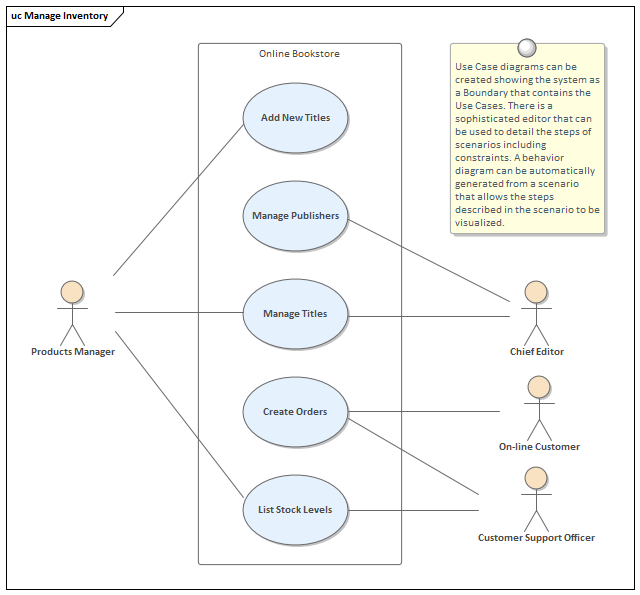
\includegraphics[width=1\textwidth]{usecase.png} 
	\caption{Use Case Model}
	\label{fig:Use Case Model}
\end{figure}

\section{Use Cases}
\textbf{Actor Definitions:}
\begin{itemize}
	\item \textbf{Procurement Managers}: These are users responsible for managing the procurement of raw materials and supplier relationships.
	\item \textbf{Logistics Managers}: These users oversee transportation, shipping, and warehouse operations.
	\item \textbf{Warehouse Managers}: They manage warehouse operations, including storage space utilization and order fulfillment.
	\item \textbf{Inventory Managers}: These users are responsible for inventory management and turnover rate analysis.
\end{itemize}
\begin{center}
	\begin{tabularx}{\textwidth}{|l|X|}
		\hline
		System & System Name \\
		\hline
		Identifier & UC-1 \\
		\hline
		Author(s) & \begin{itemize}[left=0pt]
			\item Author Name:
			\item Author Email:
		\end{itemize} \\
		\hline
		Version & 1.0 \\
		\hline
		Priority & High \\
		\hline
		Name & Analysis of the Lead Time for material procurement \\
		\hline
		Pre-Condition(s) &  \begin{itemize}[left=0pt]
			\item User has a valid account on the system.
			\item Procurement data is available in the system.
		\end{itemize} \\
		\hline
		Post-Condition(s) & \begin{itemize}[left=0pt]
			\item Lead time analysis report is generated.
		\end{itemize} \\
		\hline
		Trigger & Procurement Manager initiates the analysis. \\
		\hline
		Normal Flow & \begin{enumerate}[left=0pt]
			\item Procurement Manager logs into the system.
			\item Procurement Manager selects the lead time analysis option.
			\item Procurement Manager inputs procurement lead time data.
			\item System generates a lead time analysis report.
		\end{enumerate} \\
		\hline
		Exceptional Flow & None \\
		\hline
		Related Actor(s) & Procurement Managers \\
		\hline
		Related Use Case(s) & None \\
		\hline
		Description & Procurement Managers analyze lead times for the procurement of raw materials to identify trends and make improvements. \\
		\hline
	\end{tabularx}
\end{center}

\begin{center}
	\begin{tabularx}{\textwidth}{|l|X|}
		\hline
		System & [System Name] \\
		\hline
		Identifier & UC-2 \\
		\hline
		Author(s) & \begin{itemize}[left=0pt]
			\item Author Name:
			\item Author Email:
		\end{itemize} \\
		\hline
		Version & 1.0 \\
		\hline
		Priority & High \\
		\hline
		Name & Supplier Delivery Time Trends \\
		\hline
		Pre-Condition(s) &  \begin{itemize}[left=0pt]
			\item Valid user account in the system.
			\item Availability of supplier delivery time data.
		\end{itemize} \\
		\hline
		Post-Condition(s) & \begin{itemize}[left=0pt]
			\item Supplier delivery time trend report generated.
		\end{itemize} \\
		\hline
		Trigger & Procurement Manager initiates analysis. \\
		\hline
		Normal Flow & \begin{enumerate}[left=0pt]
			\item Procurement Manager logs in.
			\item Selects supplier delivery time trend analysis.
			\item Inputs delivery time data.
			\item System generates supplier delivery time trend.
		\end{enumerate} \\
		\hline
		Exceptional Flow & None \\
		\hline
		Related Actor(s) & Procurement Managers \\
		\hline
		Related Use Case(s) & None \\
		\hline
		Description & Procurement Managers analyze supplier delivery time trends to identify months and quarters with significant changes. \\
		\hline
	\end{tabularx}
\end{center}

\begin{center}
	\begin{tabularx}{\textwidth}{|l|X|}
		\hline
		System & [System Name] \\
		\hline
		Identifier & UC-3 \\
		\hline
		Author(s) & \begin{itemize}[left=0pt]
			\item Author Name:
			\item Author Email:
		\end{itemize} \\
		\hline
		Version & 1.0 \\
		\hline
		Priority & Moderate \\
		\hline
		Name & Shipping Cost Trend Analysis \\
		\hline
		Pre-Condition(s) &  \begin{itemize}[left=0pt]
			\item Valid user account in the system.
			\item Availability of shipping cost data.
		\end{itemize} \\
		\hline
		Post-Condition(s) & \begin{itemize}[left=0pt]
			\item Shipping cost trend report generated.
		\end{itemize} \\
		\hline
		Trigger & Logistics Manager initiates analysis. \\
		\hline
		Normal Flow & \begin{enumerate}[left=0pt]
			\item Logistics Manager logs in.
			\item Selects shipping cost trend analysis option.
			\item Inputs shipping cost data.
			\item System generates shipping cost trend report.
		\end{enumerate} \\
		\hline
		Exceptional Flow & None \\
		\hline
		Related Actor(s) & Logistics Managers \\
		\hline
		Related Use Case(s) & None \\
		\hline
		Description & None. \\
		\hline
	\end{tabularx}
\end{center}

\begin{center}
	\begin{tabularx}{\textwidth}{|l|X|}
		\hline
		System & [System Name] \\
		\hline
		Identifier & UC-4 \\
		\hline
		Author(s) & \begin{itemize}[left=0pt]
			\item Author Name:
			\item Author Email:
		\end{itemize} \\
		\hline
		Version & 1.0 \\
		\hline
		Priority & Moderate \\
		\hline
		Name & Storage Utilization Monitoring \\
		\hline
		Pre-Condition(s) &  \begin{itemize}[left=0pt]
			\item Valid user account in the system.
			\item Availability of warehouse storage data.
		\end{itemize} \\
		\hline
		Post-Condition(s) & \begin{itemize}[left=0pt]
			\item Storage utilization monitoring report generated.
		\end{itemize} \\
		\hline
		Trigger & Warehouse Manager initiates monitoring. \\
		\hline
		Normal Flow & \begin{enumerate}[left=0pt]
			\item Warehouse Manager logs in.
			\item Selects storage utilization monitoring option.
			\item Inputs storage utilization data.
			\item System generates storage utilization monitoring report.
		\end{enumerate} \\
		\hline
		Exceptional Flow & None \\
		\hline
		Related Actor(s) & Warehouse Managers \\
		\hline
		Related Use Case(s) & None \\
		\hline
		Description & [Add a brief description if needed] \\
		\hline
	\end{tabularx}
\end{center}

\begin{center}
	\begin{tabularx}{\textwidth}{|l|X|}
		\hline
		System & [System Name] \\
		\hline
		Identifier & UC-5 \\
		\hline
		Author(s) & \begin{itemize}[left=0pt]
			\item Author Name:
			\item Author Email:
		\end{itemize} \\
		\hline
		Version & 1.0 \\
		\hline
		Priority & Moderate \\
		\hline
		Name & Inventory Turnover Analysis \\
		\hline
		Pre-Condition(s) &  \begin{itemize}[left=0pt]
			\item Valid user account in the system.
			\item Availability of inventory turnover rate data.
		\end{itemize} \\
		\hline
		Post-Condition(s) & \begin{itemize}[left=0pt]
			\item Inventory turnover analysis report generated.
		\end{itemize} \\
		\hline
		Trigger & Inventory Manager initiates analysis. \\
		\hline
		Normal Flow & \begin{enumerate}[left=0pt]
			\item Inventory Manager logs in.
			\item Selects inventory turnover analysis option.
			\item Inputs turnover rate data.
			\item System generates inventory turnover analysis report.
		\end{enumerate} \\
		\hline
		Exceptional Flow & None \\
		\hline
		Related Actor(s) & Inventory Managers \\
		\hline
		Related Use Case(s) & None \\
		\hline
		Description & [Add a brief description if needed] \\
		\hline
	\end{tabularx}
\end{center}

\begin{center}
	\begin{tabularx}{\textwidth}{|l|X|}
		\hline
		System & [System Name] \\
		\hline
		Identifier & UC-6 \\
		\hline
		Author(s) & \begin{itemize}[left=0pt]
			\item Author Name:
			\item Author Email:
		\end{itemize} \\
		\hline
		Version & 1.0 \\
		\hline
		Priority & Moderate \\
		\hline
		Name & Supplier Performance Ranking \\
		\hline
		Pre-Condition(s) &  \begin{itemize}[left=0pt]
			\item Valid user account in the system.
			\item Availability of supplier performance data.
		\end{itemize} \\
		\hline
		Post-Condition(s) & \begin{itemize}[left=0pt]
			\item Supplier ranking report generated.
		\end{itemize} \\
		\hline
		Trigger & Procurement Manager initiates ranking. \\
		\hline
		Normal Flow & \begin{enumerate}[left=0pt]
			\item Procurement Manager logs in.
			\item Selects supplier performance ranking option.
			\item Utilizes inputs for supplier performance data.
			\item System generates supplier ranking report.
		\end{enumerate} \\
		\hline
		Exceptional Flow & None \\
		\hline
		Related Actor(s) & Procurement Managers \\
		\hline
		Related Use Case(s) & None \\
		\hline
		Description & [Add a brief description if needed] \\
		\hline
	\end{tabularx}
\end{center}

\begin{center}
	\begin{tabularx}{\textwidth}{|l|X|}
		\hline
		System & [System Name] \\
		\hline
		Identifier & UC-7 \\
		\hline
		Author(s) & \begin{itemize}[left=0pt]
			\item Author Name:
			\item Author Email:
		\end{itemize} \\
		\hline
		Version & 1.0 \\
		\hline
		Priority & Moderate \\
		\hline
		Name & Analyzing Popular Transportation Routes \\
		\hline
		Pre-Condition(s) &  \begin{itemize}[left=0pt]
			\item Valid user account in the system.
			\item Availability of shipment route data.
		\end{itemize} \\
		\hline
		Post-Condition(s) & \begin{itemize}[left=0pt]
			\item Route analytics report generated.
		\end{itemize} \\
		\hline
		Trigger & Logistics Manager initiates analysis. \\
		\hline
		Normal Flow & \begin{enumerate}[left=0pt]
			\item Logistics Manager logs in.
			\item Selects route analytics option.
			\item Inputs shipment route data.
			\item System generates route analytics report.
		\end{enumerate} \\
		\hline
		Exceptional Flow & None \\
		\hline
		Related Actor(s) & Logistics Managers \\
		\hline
		Related Use Case(s) & None \\
		\hline
		Description & [Add a brief description if needed] \\
		\hline
	\end{tabularx}
\end{center}

\begin{center}
	\begin{tabularx}{\textwidth}{|l|X|}
		\hline
		System & [System Name] \\
		\hline
		Identifier & UC-8 \\
		\hline
		Author(s) & \begin{itemize}[left=0pt]
			\item Author Name:
			\item Author Email:
		\end{itemize} \\
		\hline
		Version & 1.0 \\
		\hline
		Priority & Low \\
		\hline
		Name & Calculating Regional Shipping Delay \\
		\hline
		Pre-Condition(s) &  \begin{itemize}[left=0pt]
			\item Valid user account in the system.
			\item Availability of shipping delay data.
		\end{itemize} \\
		\hline
		Post-Condition(s) & \begin{itemize}[left=0pt]
			\item Regional delay analysis report generated.
		\end{itemize} \\
		\hline
		Trigger & Logistics Manager initiates analysis. \\
		\hline
		Normal Flow & \begin{enumerate}[left=0pt]
			\item Logistics Manager logs in.
			\item Selects regional delay analysis option.
			\item Inputs shipping delay data.
			\item System generates regional delay analysis report.
		\end{enumerate} \\
		\hline
		Exceptional Flow & None \\
		\hline
		Related Actor(s) & Logistics Managers \\
		\hline
		Related Use Case(s) & None \\
		\hline
		Description & [Add a brief description if needed] \\
		\hline
	\end{tabularx}
\end{center}

\begin{center}
	\begin{tabularx}{\textwidth}{|l|X|}
		\hline
		System & [System Name] \\
		\hline
		Identifier & UC-9 \\
		\hline
		Author(s) & \begin{itemize}[left=0pt]
			\item Author Name:
			\item Author Email:
		\end{itemize} \\
		\hline
		Version & 1.0 \\
		\hline
		Priority & High \\
		\hline
		Name & Assessing Inventory Stockout Risk \\
		\hline
		Pre-Condition(s) &  \begin{itemize}[left=0pt]
			\item Valid user account in the system.
			\item Availability of inventory data and demand forecasts.
		\end{itemize} \\
		\hline
		Post-Condition(s) & \begin{itemize}[left=0pt]
			\item Stockout risk assessment report generated.
		\end{itemize} \\
		\hline
		Trigger & Inventory Manager initiates assessment. \\
		\hline
		Normal Flow & \begin{enumerate}[left=0pt]
			\item Inventory Manager logs in.
			\item Selects stockout risk assessment option.
			\item Inputs inventory data and demand forecasts.
			\item System generates stockout risk assessment report.
		\end{enumerate} \\
		\hline
		Exceptional Flow & None \\
		\hline
		Related Actor(s) & Inventory Managers \\
		\hline
		Related Use Case(s) & None \\
		\hline
		Description & [Add a brief description if needed] \\
		\hline
	\end{tabularx}
\end{center}

\begin{center}
	\begin{tabularx}{\textwidth}{|l|X|}
		\hline
		System & [System Name] \\
		\hline
		Identifier & UC-10 \\
		\hline
		Author(s) & \begin{itemize}[left=0pt]
			\item Author Name:
			\item Author Email:
		\end{itemize} \\
		\hline
		Version & 1.0 \\
		\hline
		Priority & High \\
		\hline
		Name & Calculating Demand Forecast Accuracy \\
		\hline
		Pre-Condition(s) &  \begin{itemize}[left=0pt]
			\item Valid user account in the system.
			\item Availability of demand forecast and actual demand data.
		\end{itemize} \\
		\hline
		Post-Condition(s) & \begin{itemize}[left=0pt]
			\item Forecast accuracy analysis report generated.
		\end{itemize} \\
		\hline
		Trigger & Inventory Manager initiates analysis. \\
		\hline
		Normal Flow & \begin{enumerate}[left=0pt]
			\item Inventory Manager logs in.
			\item Selects demand forecast accuracy analysis option.
			\item Inputs actual demand data.
			\item System generates forecast accuracy analysis report.
		\end{enumerate} \\
		\hline
		Exceptional Flow & None \\
		\hline
		Related Actor(s) & Inventory Managers \\
		\hline
		Related Use Case(s) & None \\
		\hline
		Description & [Add a brief description if needed] \\
		\hline
	\end{tabularx}
\end{center}




